\subsection{Probe 1}

Die erste Probe zeigt eine gleichmäßige, klar abgegrenzte Struktur mit regelmäßig angeordneten quadratischen Elementen (siehe Abbildung~\ref{Abbildung 6 :probe1}). Die Reflexionssignale erscheinen homogen, ohne sichtbare Unterbrechungen oder Unregelmäßigkeiten innerhalb der Materialübergänge. Auffällig ist die hohe Signalklarheit in den bondfreien Zonen. Es lassen sich weder Risse noch Delaminationen erkennen, was auf eine saubere Verarbeitung und intakte Schichten schließen lässt.
\vspace{0.2cm}
\begin{figure}[htbp]
    \centering
    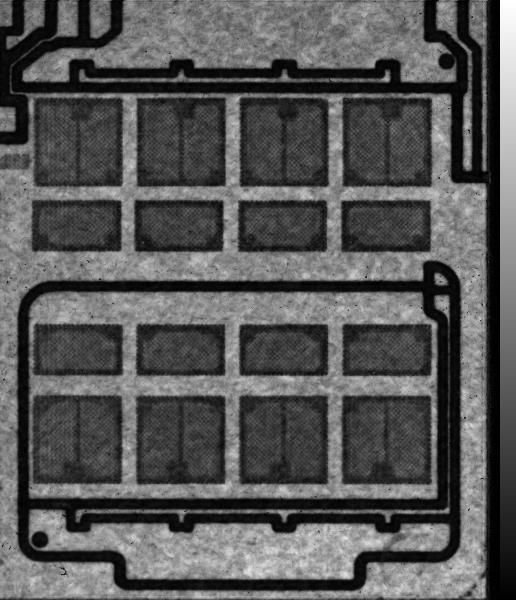
\includegraphics[scale=0.20]{Bilder/Probe11.jpg}
    \caption{C-Scan der Probe 1 mit klar erkennbaren Strukturen und homogener Reflexion.}
    \label{Abbildung 6 :probe1}
\end{figure}
\begin{figure}[htbp]
    \centering
    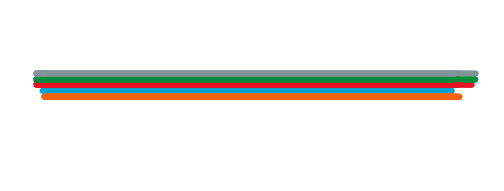
\includegraphics[scale=0.75]{Bilder/probelinie1}
    \caption{Schematische Darstellung der Materialschichten der Probe 1 (DCB-Modul) mit farblich gekennzeichneten Ebenen. Die grüne Linie stellt den gesinterten Halbleiter dar, die rote Linie die Bondschicht, die blaue Linie das Keramiksubstrat und die orange Linie die Kupferbasis.}
    \label{Abbildung 7 :Schematische Darstellung der Materialschichten der Probe 1 (DCB-Modul) mit farblich gekennzeichneten Ebenen. Die grüne Linie stellt den gesinterten Halbleiter dar, die rote Linie die Bondschicht, die blaue Linie das Keramiksubstrat und die orange Linie die Kupferbasis.}
\end{figure}
\vspace{0.5cm}
\subsection{Probe 2}
Bei der zweiten Probe wird eine Schicht-für-Schicht-Analyse durchgeführt. In den insgesamt fünf Fokusebenen zeigen sich deutliche Unterschiede in der Signalintensität und den erkennbaren Strukturen. Die obersten Ebenen (Abbildung~\ref{Abbildung 8_1:probe2_1} und \ref{Abbildung 8_2:probe2_2}) erscheinen relativ glatt, wobei eine kreisförmige Auffälligkeit in Form eines dunklen Punktes sichtbar ist. Dies könnte auf einen Lufteinschluss oder lokale Delamination hindeuten.

Mit zunehmender Tiefenlage (Abbildung~\ref{Abbildung 9_1:probe2_3} bis \ref{Abbildung 9_2:probe2_4}) treten vermehrt Leiterstrukturen hervor, die in den oberen Schichten nicht sichtbar waren. Zudem zeigen sich in tieferen Ebenen leichte Schattenbildungen und Signalbrüche entlang einzelner Linien, was auf potenzielle Trennungen oder Materialunregelmäßigkeiten in unteren Bondschichten hinweist.
\vspace{0.2cm}
\begin{figure}[htbp]
    \centering
    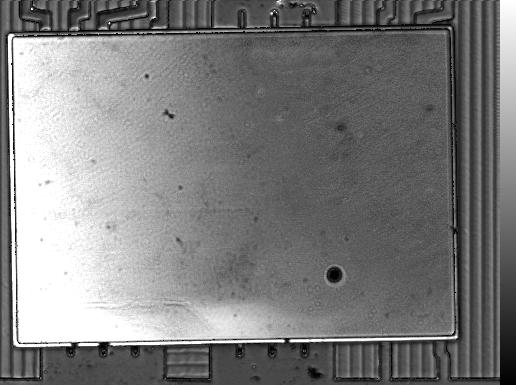
\includegraphics[scale=0.30]{Bilder/Probe2_i794_x001.jpg}
    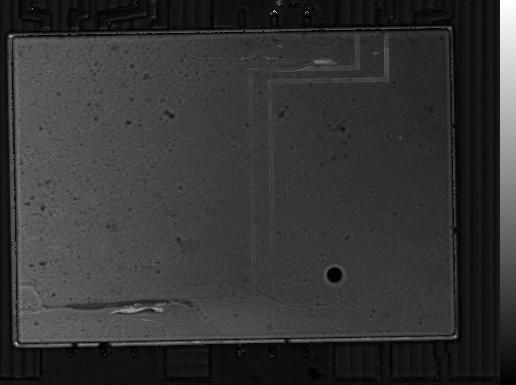
\includegraphics[scale=0.30]{Bilder/Probe2_i794_x002.jpg}
    \caption{Obere Fokusebenen der Probe 2. Die rechte Abbildung zeigt eine auffällige Reflexionsunterbrechung.}
    \label{Abbildung 8_1:probe2_1}
    \label{Abbildung 8_2:probe2_2}
\end{figure}

\begin{figure}[htbp]
    \centering
    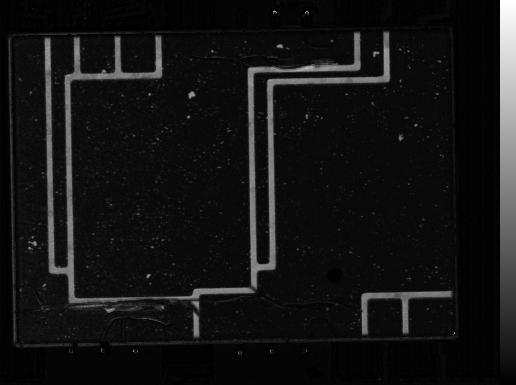
\includegraphics[scale=0.30]{Bilder/Probe2_i794_x003.jpg}
    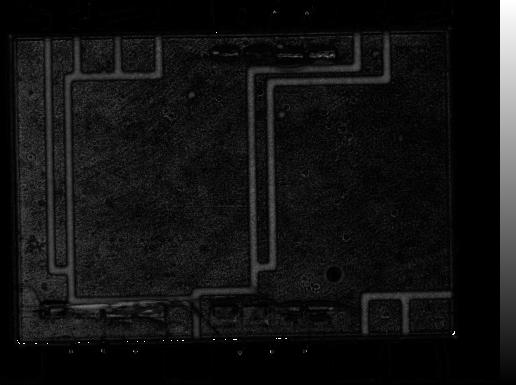
\includegraphics[scale=0.30]{Bilder/Probe2_i794_x004.jpg}
    \caption{Mittlere Fokusebenen der Probe 2 mit zunehmender Sichtbarkeit der Leiterstrukturen.}
    \label{Abbildung 9_1:probe2_3}
    \label{Abbildung 9_2:probe2_4}
\end{figure}
\clearpage
\begin{figure}[htbp]
    \centering
    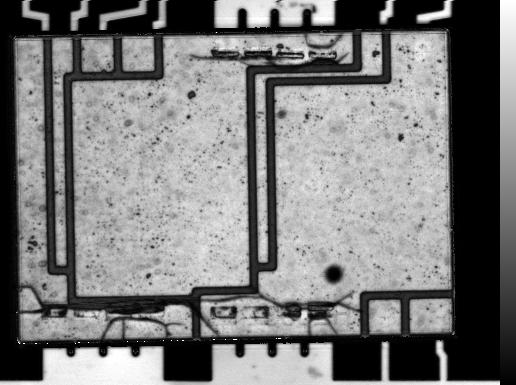
\includegraphics[scale=0.30]{Bilder/Probe2_i794_x005.jpg}
    \caption{Tiefste gescannte Ebene der Probe 2. Sichtbare Leiterbahnen mit lokalen Unregelmäßigkeiten im unteren Bereich.}
    \label{Abbildung 10:probe2_5}
\end{figure}
\begin{figure}[htbp]
    \centering
    
\includegraphics[scale=0.75]{Bilder/probelinie2}
    \caption{Visualisierung der in mehreren Fokusebenen gescannten Schichten der Probe 2. Die graue Linie zeigt die Oberfläche bzw. Metallabdeckung, die roten Linien markieren Bond- oder Kontaktzonen, die orange Linie kennzeichnet Kupferleiterbahnen, und die blaue Linie stellt das keramische Substrat dar.}
    \label{Abbildung 11 :Visualisierung der in mehreren Fokusebenen gescannten Schichten der Probe 2. Die graue Linie zeigt die Oberfläche bzw. Metallabdeckung, die roten Linien markieren Bond- oder Kontaktzonen, die orange Linie kennzeichnet Kupferleiterbahnen, und die blaue Linie stellt das keramische Substrat dar.}
\end{figure}

\subsection{Probe 3}

In der letzten Probe, einem DoL-Modul, fällt sofort die großflächige, glatte Reflexionsfläche auf (siehe Abbildung~\ref{Abbildung 12:probe3}). Die Struktur wirkt weitgehend homogen. Es sind keine offensichtlichen Risse oder Hohlräume erkennbar. Bemerkenswert ist jedoch die gute Lesbarkeit des Schriftzugs \enquote{FH-KIEL} in der Bildmitte. Dies deutet auf eine hohe Oberflächengüte und gleichmäßige Signalreflexion hin.
\vspace{0.2cm}
\begin{figure}[htbp]
    \centering
    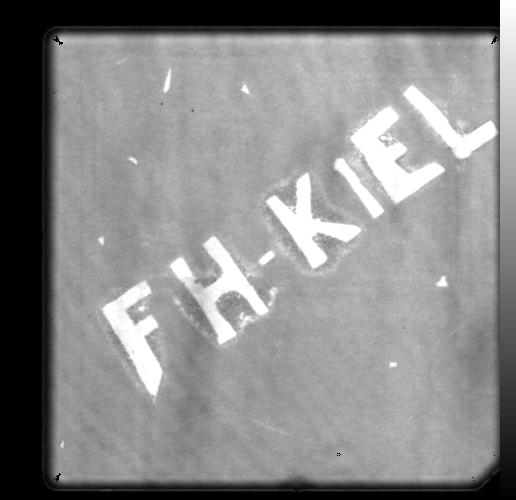
\includegraphics[scale=0.30]{Bilder/Probe3_i795_c.jpg}
    \caption{C-Scan der Probe 3 (DoL-Modul) mit gleichmäßiger Reflexionsfläche und klar erkennbarer Gravurstruktur.}
    \label{Abbildung 12:probe3}
\end{figure}
\begin{figure}[htbp]
    \centering
    
\includegraphics[scale=0.75]{Bilder/probelinie3}
    \caption{Schichtdarstellung der Probe 3 (DoL-Modul) mit farblich codierten Materialien. Die schwarze Linie stellt die Metallkappe dar, die violette Linie steht für die organische Trägerfolie und die orange Linie kennzeichnet die eingebetteten Kupferstrukturen.}
    \label{Abbildung 13 :Schichtdarstellung der Probe 3 (DoL-Modul) mit farblich codierten Materialien. Die schwarze Linie stellt die Metallkappe dar, die violette Linie steht für die organische Trägerfolie und die orange Linie kennzeichnet die eingebetteten Kupferstrukturen.}
\end{figure}